\section{Metodologia}
\label{sec:metodologia}

A metodologia proposta fundamenta-se na análise sistemática de metadados de tabelas \textit{Apache Iceberg} para tomada de decisões sobre o ambiente de execução mais adequado, resultando em melhor custo-benefício no processamento. O sistema proposto, denominado \textit{DyraSQL}, implementa roteamento dinâmico de consultas SQL baseado em metadados.

\subsection{Arquitetura da Solução Proposta}

O \textit{DyraSQL} implementa uma arquitetura que integra múltiplos componentes para análise de consultas e direcionamento automático para \textit{clusters} com capacidades distintas. A arquitetura é composta por quatro componentes principais que trabalham de forma integrada, direcionando consultas leves para \textit{clusters} menores e consultas pesadas para infraestrutura mais robusta. O \textit{Query Analyzer} executa o comando \textit{EXPLAIN (TYPE IO)} do \textit{Trino} para extrair metadados sobre volume de dados, custos de I/O e características das consultas, incluindo tamanho estimado dos dados de saída, número estimado de linhas, custo de CPU e informações sobre filtros aplicados. O \textit{Decision Engine} aplica o algoritmo de pontuação baseado nos metadados extraídos para determinar o ambiente de execução mais adequado (\textit{small}, \textit{medium} ou \textit{large}). O \textit{Trino Gateway Proxy} intercepta consultas SQL e integra-se com o \textit{DyraSQL Core} para obter decisões de roteamento, direcionando a consulta para o \textit{cluster} selecionado através do \textit{Trino Gateway} oficial. O \textit{Monitoring System} coleta métricas de execução e atualiza o histórico para aprendizado contínuo.

\begin{figure}[ht]
	\centering
	\caption{Contexto do Sistema - DyraSQL}
	\label{fig:contexto-sistema}
	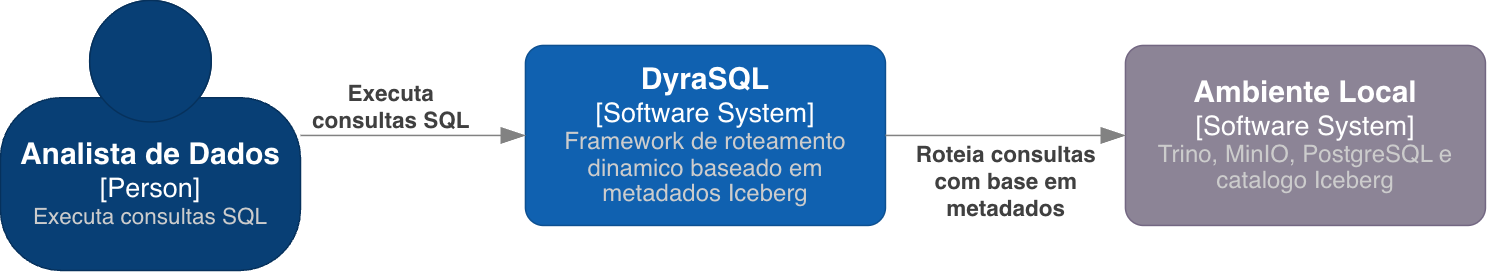
\includegraphics[width=0.9\textwidth]{figuras/contexto.png}\\
	\fonte{Elaborado pelo autor.}
\end{figure}
\FloatBarrier

A Figura \ref{fig:contexto-sistema} apresenta o contexto do \textit{DyraSQL}, mostrando como o sistema se relaciona com usuários e com o ambiente de execução local. O analista de dados executa consultas SQL que são processadas pelo \textit{DyraSQL}, que utiliza \textit{clusters} \textit{Trino} e o \textit{data lake} local para roteamento.

\begin{figure}[ht]
	\centering
	\caption{Containers do Sistema - \textit{DyraSQL}}
	\label{fig:containers-sistema}
	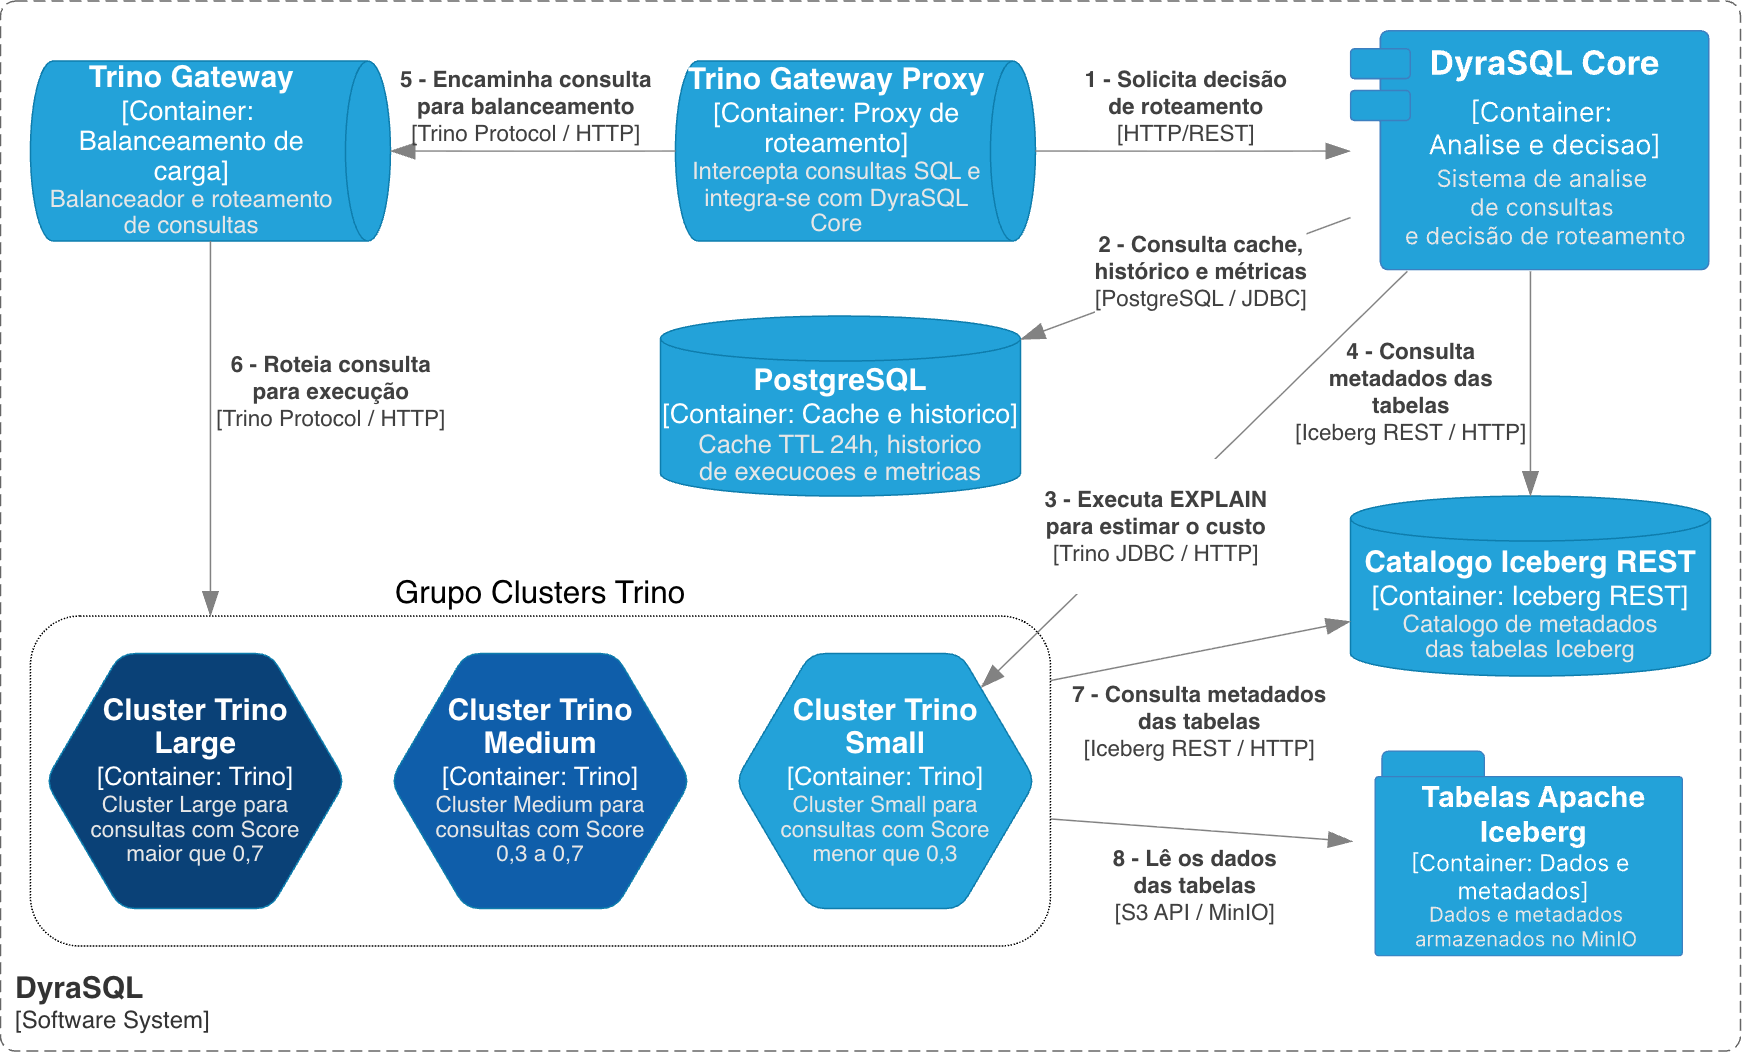
\includegraphics[width=0.9\textwidth]{figuras/container.png}\\
	\fonte{Elaborado pelo autor.}
\end{figure}
\FloatBarrier

A Figura \ref{fig:containers-sistema} detalha a arquitetura de containers do \textit{DyraSQL}, evidenciando os principais componentes, sendo que o \textit{Trino Gateway Proxy} é responsável pela interceptação de consultas e integração com o \textit{DyraSQL Core}, o \textit{Trino Gateway} oficial atua como balanceador, o \textit{DyraSQL Core} realiza a análise de consultas utilizando \textit{EXPLAIN (TYPE IO)} e a decisão de roteamento, e os \textit{clusters} de execução realizam o processamento. A integração com PostgreSQL permite o armazenamento de histórico e \textit{cache} de decisões, enquanto o acesso aos metadados é realizado através do comando \textit{EXPLAIN (TYPE IO)} do \textit{Trino} sobre tabelas no MinIO. Os três \textit{containers Trino} representados na Figura \ref{fig:containers-sistema}, denominados \textit{cluster large}, \textit{cluster medium} e \textit{cluster small}, correspondem às três faixas de capacidade descritas na Seção~\ref{sec:algoritmo-decisao}, sendo cada um configurado com limites distintos de memória e paralelismo dentro do ambiente Docker Compose e acessando igualmente o mesmo Catálogo Iceberg REST, o que garante consistência dos dados independentemente do \textit{container} selecionado.

\begin{figure}[ht]
	\centering
	\caption{Componentes do \textit{DyraSQL} Core}
	\label{fig:componentes-sistema}
	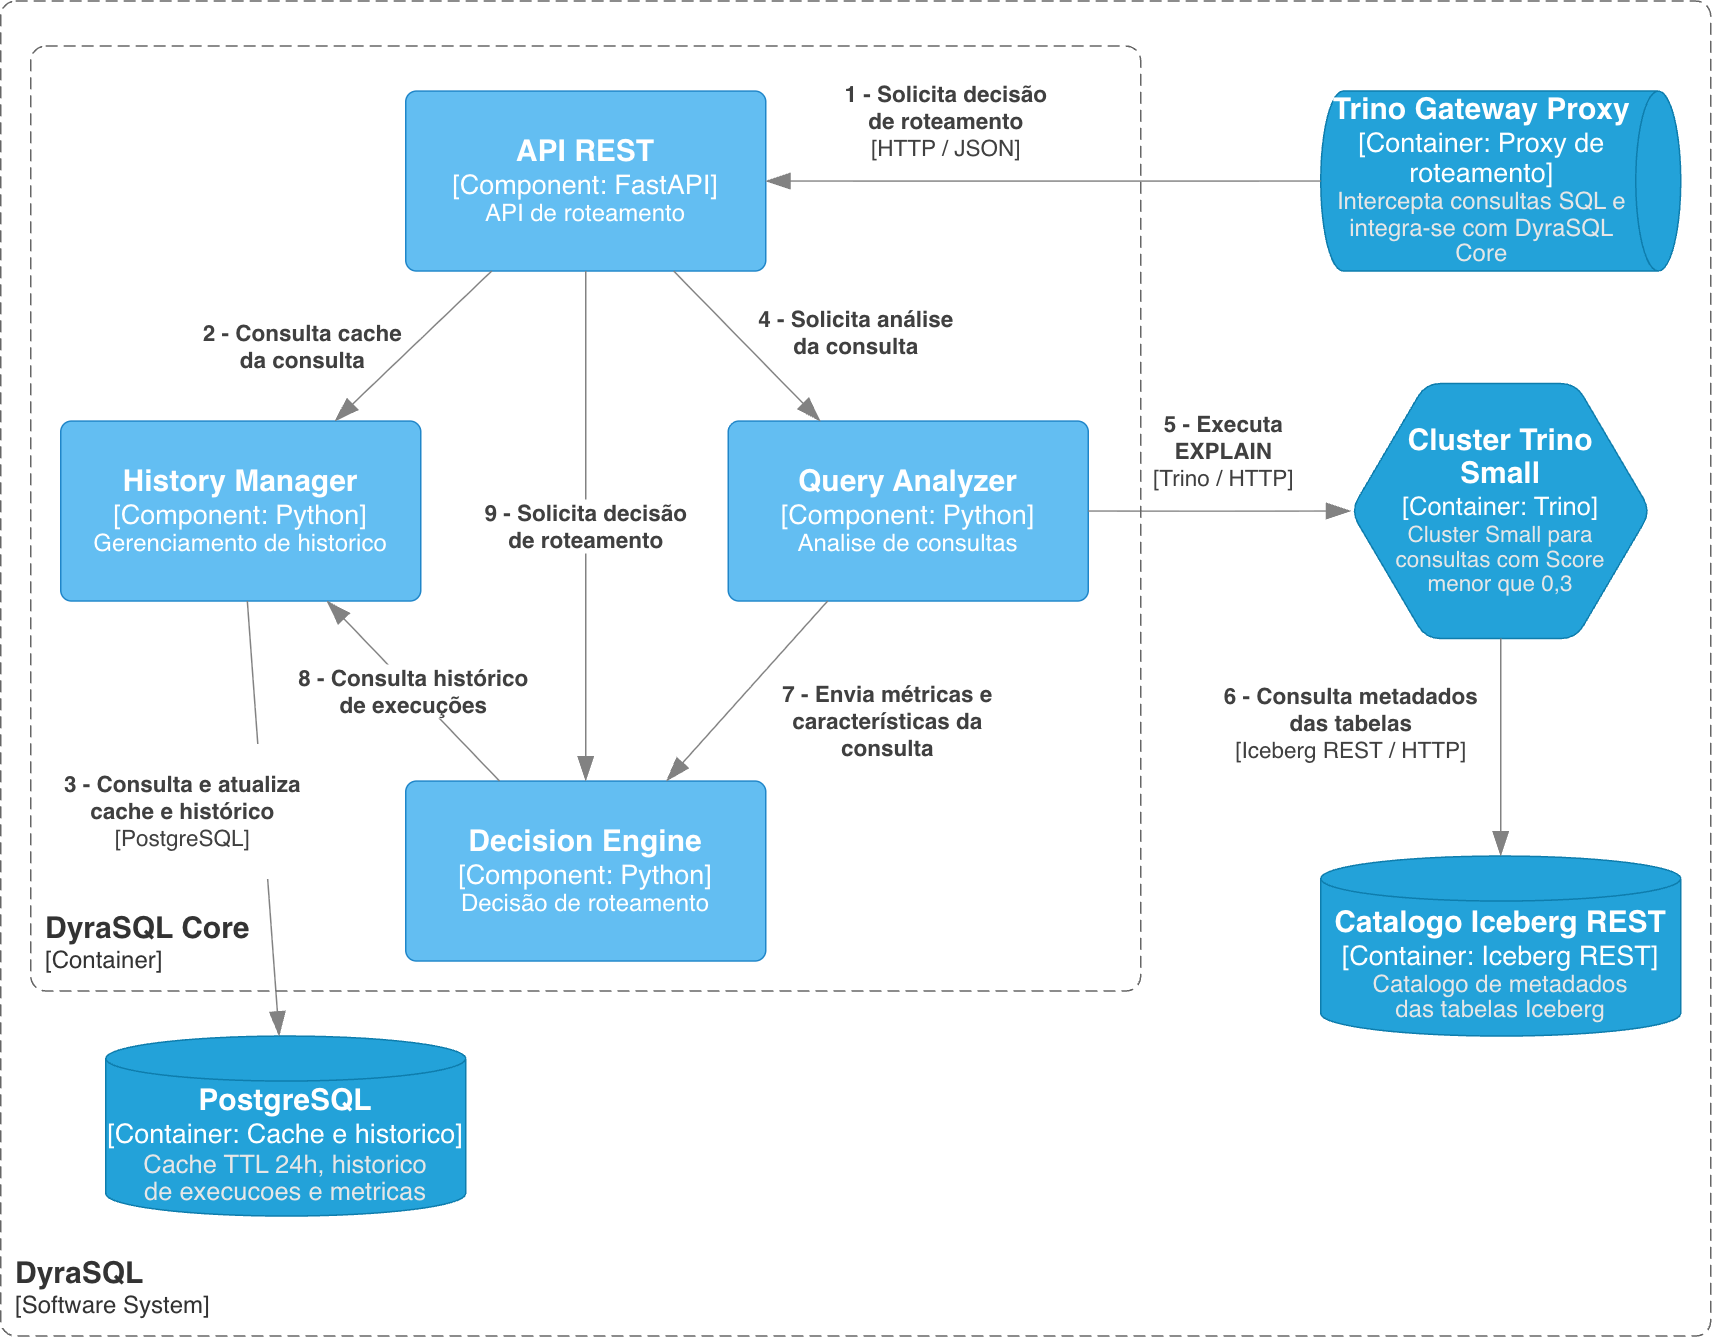
\includegraphics[width=0.9\textwidth]{figuras/componentes.png}\\
	\fonte{Elaborado pelo autor.}
\end{figure}
\FloatBarrier

A Figura \ref{fig:componentes-sistema} apresenta os componentes internos do \textit{DyraSQL Core}, demonstrando o fluxo de dados desde a interceptação da consulta até a execução no \textit{cluster} selecionado e o \textit{feedback} para o histórico. A arquitetura evidencia a integração entre os componentes do sistema, sendo que cada módulo contribui para o processo de tomada de decisão baseado em metadados.

\subsection{Extração de Metadados Relevantes}

O \textit{DyraSQL} utiliza o comando \textit{EXPLAIN (TYPE IO)} do \textit{Trino} para extrair informações sobre o volume de dados e custos de I/O que serão processados por cada consulta SQL. Esta abordagem aproveita a capacidade do \textit{Trino} de analisar consultas antes da execução, fornecendo estimativas baseadas no plano de execução. O \textit{EXPLAIN (TYPE IO)} retorna informações estruturadas em formato \textit{JSON} contendo os metadados necessários para o Algoritmo de decisão, sendo que o sistema extrai especificamente \textit{outputSizeInBytes}, tamanho estimado dos dados de saída em \textit{bytes}, já considerando filtros aplicados; \textit{outputRowCount}, número estimado de linhas; \textit{cpuCost}, custo estimado de processamento; e \textit{columnConstraints}, informações sobre filtros aplicados nas colunas. A Tabela \ref{tab:siglas-calculo} apresenta as siglas utilizadas nos cálculos do Algoritmo de decisão.

\begin{table}[ht]
	\centering
	\caption{Siglas Utilizadas nos Cálculos do Algoritmo de Decisão}
	\label{tab:siglas-calculo}
	\begin{tabular}{ll}
	\hline
	\textbf{Sigla} & \textbf{Descrição} \\
	\hline
	$S$ & \textit{Score} final do Algoritmo de decisão \\
	$f_v$ & Fator de volume normalizado \\
	$f_c$ & Fator de complexidade normalizado \\
	$f_h$ & Fator histórico normalizado \\
	$w_1$ & Peso do Fator volume \\
	$w_2$ & Peso do Fator complexidade \\
	$w_3$ & Peso do Fator histórico \\
	$T_e$ & Tamanho efetivo em GB (obtido de \textit{outputSizeInBytes}) \\
	$R_e$ & Número de linhas efetivas (obtido de \textit{outputRowCount}) \\
	$C_e$ & Custo de CPU efetivo (obtido de \textit{cpuCost}) \\
	$T_{max}$ & Limite máximo de tamanho em GB \\
	$R_{max}$ & Limite máximo de linhas \\
	$F_o$ & Fator de ajuste \\
	$J$ & Número de JOINs \\
	$Ag$ & Número de agregações \\
	$S_q$ & Número de subconsultas \\
	$F_p$ & Número de filtros particionados \\
	$F_{np}$ & Número de filtros não-particionados \\
	$L_c$ & Limite de complexidade \\
	$S_p$ & \textit{Score} prévio da mesma consulta \\
	\hline
	\end{tabular}
	\fonte{Elaborado pelo autor.}
\end{table}
\FloatBarrier

A Tabela \ref{tab:siglas-calculo} apresenta as variáveis utilizadas no Algoritmo de decisão, organizadas desde o \textit{Score} final até os parâmetros específicos de cada fator. Esta padronização uniformiza a notação matemática utilizada nas fórmulas do Algoritmo, facilitando a compreensão dos cálculos nas seções subsequentes. Com essas variáveis definidas, é possível demonstrar a aplicação prática da metodologia através de um exemplo concreto de consulta SQL.

\subsection{Consulta SQL de Referência}

Para demonstrar a aplicação prática da metodologia, considera-se a consulta SQL apresentada no Algoritmo \ref{alg:consulta-vendas}, que processa a Tabela \ref{tab:dataset-teste}. A escolha dessa consulta como referência não é arbitrária, sendo que sua estrutura combina, deliberadamente, um volume de dados moderado, filtro por coluna particionada e complexidade estrutural intermediária, de modo que os três fatores do Algoritmo de decisão, volume, complexidade e histórico, contribuam de forma perceptível para o \textit{Score} final. Consultas mais simples, sem \textit{JOIN} ou agregações, tenderiam a produzir Fator de complexidade próximo de zero, mascarando a contribuição relativa do Fator volume no cálculo, o que motivou a seleção de uma consulta com complexidade intermediária para fins de demonstração.

\begin{table}[ht]
	\centering
	\caption{Dataset de Teste}
	\label{tab:dataset-teste}
	\begin{tabular}{ll}
	\hline
	\textbf{Característica} & \textbf{Descrição} \\
	\hline
	Formato & \textit{Apache Iceberg} \\
	Armazenamento & MinIO \\
	Tamanho aproximado & Até 10 GB \\
	Particionamento & Coluna \textit{date} (função \textit{day}) \\
	Origem & Tabela sintética gerada no ambiente local \\
	\hline
	\textbf{Colunas} & \textbf{Tipo} \\
	\hline
	\textit{tenant\_id} & string \\
	status & string \\
	valor & double \\
	\textit{date} & timestamp \\
	\textit{created\_at} & timestamp \\
	\textit{updated\_at} & timestamp \\
	document & string (\textit{JSON}) \\
	\textit{surrogate\_key} & string \\
	\hline
	\end{tabular}
	\fonte{Elaborado pelo autor.}
\end{table}
\FloatBarrier

A Tabela \ref{tab:dataset-teste} apresenta as características do \textit{dataset} utilizado para demonstração da metodologia proposta, sendo que o formato \textit{Apache Iceberg} permite particionamento por \textit{date}, facilitando a aplicação de filtros que reduzem o volume efetivo de dados processados. O armazenamento no MinIO e o tamanho de até 10 GB representam um cenário controlado para execução local, dimensionado para caber na memória disponível da máquina utilizada nos experimentos, sendo que o particionamento pela função \textit{day} aplicada à coluna \textit{date} permite que o sistema processe apenas frações relevantes dos dados através de filtros temporais. Os registros foram gerados por um script de dados sintéticos, executado continuamente por um período determinado, simulando o crescimento incremental de um \textit{data lake} em produção.

\begin{algorithm}[ht]
\caption{Consulta de Análise de Dados}
\label{alg:consulta-vendas}
\begin{algorithmic}[1]
\REQUIRE Tabela \textit{Apache Iceberg} no MinIO (Tabela \ref{tab:dataset-teste})
\ENSURE Relatório agregado por tenant e período
\STATE SELECT t.tenant\_id, t.categoria, COUNT(*) as total\_registros
\STATE SUM(d.valor) as valor\_total, AVG(d.valor) as valor\_medio
\STATE FROM dados d
\STATE JOIN tenant\_info t ON d.tenant\_id = t.tenant\_id
\STATE WHERE d.date >= '2024-01-01' AND d.date < '2024-02-01'
\STATE AND d.status = 'ATIVO'
\STATE AND t.categoria IN (SELECT categoria FROM tenant\_info WHERE nivel > (SELECT AVG(nivel) FROM tenant\_info))
\STATE GROUP BY t.tenant\_id, t.categoria
\STATE HAVING COUNT(*) > 100
\STATE ORDER BY valor\_total DESC
\STATE LIMIT 50;
\end{algorithmic}
\end{algorithm}
\FloatBarrier

Esta consulta possui 1 JOIN com tabela de dimensão (tenant\_info) utilizando a chave tenant\_id, 3 agregações (COUNT, SUM, AVG), 2 subconsultas e filtros por data e status. O sistema analisa a complexidade estrutural da consulta, identificando operações que requerem processamento distribuído. O filtro por data na coluna particionada permite que o sistema processe apenas uma fração dos dados armazenados, sendo que o \textit{range} da cláusula WHERE determina a quantidade efetiva de dados a serem lidos.

\subsection{Algoritmo de Decisão de Roteamento}
\label{sec:algoritmo-decisao}

O Algoritmo de decisão implementa uma abordagem baseada em pontuação que combina metadados extraídos com características da consulta SQL. O processo opera em duas fases principais, sendo que a primeira é a verificação de \textit{cache}, que consulta o PostgreSQL para verificar se existe uma decisão recente para a mesma \textit{query fingerprint}, e a segunda é o cálculo dinâmico, que executa análise completa dos metadados quando não há \textit{cache} válido. O \textit{fingerprint} é obtido normalizando a consulta SQL original (letras minúsculas, espaços colapsados e literais substituídos por um marcador genérico) e aplicando a função \textit{hash} SHA-256 sobre o resultado, de modo que consultas estruturalmente idênticas com valores de filtro distintos produzam o mesmo \textit{fingerprint} e reaproveitem o \textit{cache}.

O \textit{DyraSQL} mantém um \textit{cache} temporal no PostgreSQL com \textit{TTL} (\textit{Time To Live}) de 24 horas, considerando que o volume de dados pode crescer através de ingestões. Para consultas com \textit{fingerprint} similar executadas nas últimas 24 horas, o sistema recupera diretamente a decisão de roteamento armazenada, eliminando a necessidade de re-análise dos metadados. Quando o \textit{cache} expira ou não existe, o sistema executa o comando \textit{EXPLAIN (TYPE IO)} no \textit{Trino} para obter informações sobre o volume de dados e custos de I/O. O Algoritmo então considera três fatores para determinar a arquitetura mais adequada, sendo que o primeiro é o volume de dados, baseado no campo \textit{outputSizeInBytes} retornado pelo \textit{EXPLAIN (TYPE IO)}, o segundo é a complexidade da consulta, analisando número de JOINs, agregações e subconsultas, e o terceiro é o histórico de execução, utilizando padrões de consultas similares. A Pontuação é calculada através da Equação \ref{eq:pontuacao}.

\begin{equation}
\label{eq:pontuacao}
S = w_1 \times f_v + w_2 \times f_c + w_3 \times f_h
\end{equation}

Com base no \textit{Score} calculado, as consultas são direcionadas para diferentes arquiteturas, sendo que \textit{Scores} menores que 0,3 são direcionados para o \textit{cluster small}, \textit{Scores} entre 0,3 e 0,7 para o \textit{cluster medium}, e \textit{Scores} maiores que 0,7 para o \textit{cluster large}. O sistema pode ajustar os pesos baseado no histórico de custo e \textit{performance} das decisões tomadas, aprendendo qual arquitetura oferece melhor relação entre custo e \textit{performance} para cada tipo de consulta.

\subsubsection{Exemplo Prático de Cálculo}

Para demonstrar o funcionamento do Algoritmo, considera-se o Algoritmo \ref{alg:consulta-vendas} executado sobre a Tabela \ref{tab:dataset-teste}. O sistema executa \textit{EXPLAIN (TYPE IO)} no \textit{Trino}, que retorna informações sobre o volume efetivo de dados a serem processados, já considerando os filtros aplicados. Para este exemplo, o \textit{EXPLAIN (TYPE IO)} retorna \textit{outputSizeInBytes} de aproximadamente 1,25 GB (1.342.177.280 \textit{bytes}) e \textit{outputRowCount} de aproximadamente 2.500.000 linhas, indicando que apenas uma fração dos dados seria processada devido ao filtro por \textit{date} na coluna particionada. No ambiente local o volume absoluto é menor, porém a mesma normalização se aplica, sendo que o exemplo numérico ilustra o cálculo independentemente da escala do \textit{warehouse}.

O Fator volume é calculado através da Equação \ref{eq:fator-volume}, sendo que o sistema utiliza os dados retornados pelo \textit{EXPLAIN (TYPE IO)}, normalizando separadamente o tamanho em GB e o número de linhas usando logaritmos, e combina os valores normalizados com pesos de 0,6 para tamanho e 0,4 para linhas, aplicando um fator de 0,1.

\begin{equation}
\label{eq:fator-volume}
f_v = \left( \frac{\log(T_e)}{\log(T_{max})} \times 0,6 + \frac{\log(R_e)}{\log(R_{max})} \times 0,4 \right) \times (1 - F_o)
\end{equation}

Para o exemplo, o \textit{EXPLAIN (TYPE IO)} retorna tamanho de 1,25 GB ($T_e = 1,25$) e aproximadamente 2.500.000 linhas ($R_e = 2.500.000$), com $T_{max} = 1000$ GB, $R_{max} = 10^9$ e $F_o = 0,1$, resultando em normalização de tamanho de 0,03 e normalização de linhas de 0,71, calculando o Fator volume através da Equação \ref{eq:fator-volume-exemplo}.

\begin{equation}
\label{eq:fator-volume-exemplo}
f_v = \left( \frac{\log(1,25)}{\log(1000)} \times 0,6 + \frac{\log(2500000)}{\log(10^9)} \times 0,4 \right) \times 0,9 = (0,03 \times 0,6 + 0,71 \times 0,4) \times 0,9 = 0,27
\end{equation}

A análise estrutural da consulta é realizada por meio da biblioteca \textit{sqlglot}, que converte o texto SQL em uma árvore de sintaxe abstrata, permitindo identificar precisamente o número de \textit{JOINs}, as agregações da lista de projeção do \textit{SELECT} principal, as subconsultas e os filtros do \textit{WHERE} de nível superior agrupados pela coluna referenciada, evitando ambiguidades de uma análise baseada em expressões regulares (como contabilizar duplamente uma agregação repetida em \textit{HAVING}). Para a consulta do Algoritmo \ref{alg:consulta-vendas}, essa análise identifica 1 JOIN, 3 agregações, 2 subconsultas, 1 filtro particionado e 2 não-particionados. Este cálculo considera a complexidade das operações SQL para determinar o nível de recursos computacionais necessários, sendo calculado através da Equação \ref{eq:fator-complexidade}.

\begin{equation}
\label{eq:fator-complexidade}
f_c = \frac{1 \times 0.2 + 3 \times 0.15 + 2 \times 0.25 + 1 \times 0.02 + 2 \times 0.1}{2.0} = 0.69
\end{equation}

Os coeficientes atribuídos a cada elemento estrutural, como 0,2 por \textit{JOIN} e 0,25 por subconsulta, não derivam de um estudo estatístico sobre custo real de execução, mas são parâmetros configuráveis conforme regras de negócio de cada organização, devendo ser calibrados de acordo com o perfil de \textit{workload} de cada ambiente de implantação.

O Fator histórico é calculado baseado no histórico de execuções anteriores da mesma consulta (mesmo \textit{fingerprint}). Quando não há histórico disponível, o sistema utiliza um valor \textit{default} de $f_h = 0,5$, representando neutralidade na decisão. Quando há histórico, o Fator histórico é determinado conforme a Tabela \ref{tab:fator-historico}, sendo que o sistema verifica se a execução anterior foi bem-sucedida, utilizando o Score prévio ($f_h = S_p$) em caso de sucesso, ou o complemento do Score prévio ($f_h = 1 - S_p$) em caso de falha. Para o exemplo em questão, considerando que não há histórico disponível, o Fator histórico assume o valor \textit{default}. Com pesos ($w_1 = 0.5$, $w_2 = 0.3$, $w_3 = 0.2$), o Score final é calculado através da Equação \ref{eq:score-final}.

\begin{table}[ht]
	\centering
	\caption{Cálculo do Fator Histórico}
	\label{tab:fator-historico}
	\begin{tabular}{ll}
	\hline
	\textbf{Condição} & \textbf{Valor de $f_h$} \\
	\hline
	Sem histórico disponível & $0,5$ \\
	Execução anterior bem-sucedida & $S_p$ \\
	Execução anterior falhou & $1 - S_p$ \\
	\hline
	\end{tabular}
	\fonte{Elaborado pelo autor.}
\end{table}
\FloatBarrier

\begin{equation}
\label{eq:score-final}
S = 0.5 \times 0.27 + 0.3 \times 0.69 + 0.2 \times 0.5 = 0.44
\end{equation}

Com \textit{Score} de 0,44, a consulta é direcionada para o \textit{cluster medium} (faixa 0,3 a 0,7). Os pesos podem ser ajustados com base no histórico de custo e \textit{performance} das decisões, inspirado em sistemas como o Amazon Redshift MDDL \cite{ding2024}. O Algoritmo principal do \textit{DyraSQL} pode ser expresso através do pseudocódigo apresentado no Algoritmo \ref{alg:roteamento-dinamico}, sendo que este processo garante que cada consulta seja direcionada para o ambiente mais adequado baseado na análise dos metadados obtidos através do \textit{EXPLAIN (TYPE IO)} do \textit{Trino}.

\begin{algorithm}[ht]
\caption{Algoritmo de Roteamento Dinâmico de Consultas}
\label{alg:roteamento-dinamico}
\begin{algorithmic}[1]
\REQUIRE consulta SQL, acesso ao \textit{Trino} para \textit{EXPLAIN (TYPE IO)}, histórico PostgreSQL
\ENSURE cluster selecionado, score calculado
    \STATE Gerar \textit{fingerprint} único da consulta SQL
    \STATE Consultar \textit{cache} no PostgreSQL usando o \textit{fingerprint}
    \STATE \textbf{Se} decisão existe no \textit{cache} \textbf{e} TTL é válido \textbf{então}
    \STATE \quad \textbf{Retornar} cluster armazenado no \textit{cache}
    \STATE \textbf{Fim se}
    \STATE Executar \textit{EXPLAIN (TYPE IO)} no \textit{Trino} para obter metadados
    \STATE Extrair \textit{outputSizeInBytes}, \textit{outputRowCount} e \textit{columnConstraints}
    \STATE Normalizar fator de volume baseado em \textit{outputSizeInBytes}
    \STATE Analisar complexidade da consulta SQL
    \STATE Consultar histórico de consultas similares
    \STATE Calcular score usando fórmula ponderada
    \STATE \textbf{Se} score é menor que 0,3 \textbf{então}
    \STATE \quad Selecionar cluster small
    \STATE \textbf{Senão se} score está entre 0,3 e 0,7 \textbf{então}
    \STATE \quad Selecionar cluster medium
    \STATE \textbf{Senão}
    \STATE \quad Selecionar cluster large
    \STATE \textbf{Fim se}
    \STATE Salvar decisão no histórico do PostgreSQL
    \STATE \textbf{Retornar} cluster selecionado
\end{algorithmic}
\end{algorithm}
\FloatBarrier

O pseudocódigo demonstra o fluxo completo do Algoritmo, desde a interceptação da consulta até a decisão final de roteamento, incluindo verificação de \textit{cache}, execução do \textit{EXPLAIN (TYPE IO)} para extração de metadados, cálculo do \textit{Score} e seleção do \textit{cluster} apropriado.

\subsection{Sistema de Histórico e Aprendizado}

O \textit{DyraSQL} mantém um histórico de execuções no PostgreSQL, armazenando \textit{fingerprints} de consultas, métricas de custo-benefício e decisões de roteamento. A cada execução de consulta, o sistema pode coletar métricas pós-execução incluindo tempo de execução, custo operacional e eficácia da decisão, salvando essas informações para enriquecimento do histórico. A eficácia é avaliada pela comparação entre o tempo observado e o esperado para a faixa de capacidade, sendo que decisões recorrentemente inadequadas podem indicar a necessidade de ajuste dos pesos $w_1$, $w_2$ e $w_3$ da Equação \ref{eq:pontuacao}.

\subsubsection{Cálculo do Fator Histórico}

O Fator histórico é calculado através da análise do histórico de execuções anteriores da mesma consulta, identificada pelo \textit{fingerprint} único gerado a partir da estrutura da consulta SQL. O sistema consulta o PostgreSQL para verificar se existe uma execução anterior da mesma consulta, sendo que quando não há histórico disponível, o sistema utiliza um valor \textit{default} de $f_h = 0,5$, representando neutralidade na decisão.

Quando há histórico disponível, o sistema verifica se a execução anterior foi bem-sucedida. Se a execução anterior foi bem-sucedida, o Fator histórico utiliza o Score prévio calculado para a mesma consulta ($f_h = S_p$). Se a execução anterior falhou, o Fator histórico utiliza o complemento do Score prévio ($f_h = 1 - S_p$), indicando que a decisão anterior não foi adequada e sugerindo uma arquitetura alternativa.

O Fator histórico é então determinado conforme a Tabela \ref{tab:fator-historico}, sendo que esta abordagem permite que o sistema aprenda com execuções anteriores da mesma consulta. Esta abordagem é inspirada em mecanismos de \textit{learned cost models} implementados em sistemas como o Amazon Redshift \cite{ding2024}. O sistema mantém um \textit{cache} temporal no PostgreSQL com \textit{TTL} de 24 horas, sendo que consultas com \textit{fingerprint} similar executadas nas últimas 24 horas recuperam diretamente a decisão de roteamento armazenada.

\subsection{Integração com \textit{Trino Gateway}}

A solução integra-se ao \textit{Trino} Gateway oficial através de uma arquitetura modular composta por três componentes principais. O primeiro componente é o \textit{Trino} Gateway oficial, compilado a partir do código-fonte em Java, que atua como balanceador e \textit{gateway} de roteamento, utilizando PostgreSQL para persistência de configurações e histórico de \textit{backends}. O segundo componente é o \textit{Trino Gateway Proxy}, desenvolvido em Python utilizando FastAPI, que intercepta consultas SQL antes do roteamento e integra-se com o \textit{DyraSQL Core} para obter decisões baseadas em análise de metadados. O terceiro componente é o \textit{DyraSQL Core}, que implementa o Algoritmo de decisão e fornece a API REST para análise de consultas e cálculo de \textit{scores}. O \textit{Trino Gateway Proxy} consulta o \textit{DyraSQL Core} através do \textit{endpoint} POST /api/v1/route para cada consulta recebida, obtendo a decisão de roteamento com \textit{cluster} recomendado, \textit{score} calculado e fatores utilizados, e então direciona a consulta para o \textit{cluster Trino} apropriado. Esta arquitetura modular permite integração com o \textit{Trino} Gateway oficial sem necessidade de modificações no código-fonte do \textit{gateway}.

O contrato do \textit{endpoint} POST /api/v1/route recebe um objeto \textit{JSON} com a consulta SQL e retorna a decisão de roteamento (\textit{cluster}, \textit{score} e fatores utilizados), conforme exemplo de requisição e resposta apresentado no Apêndice A.

\subsection{Implementação do \textit{framework}}

O \textit{framework DyraSQL} foi desenvolvido utilizando Python para os módulos de roteamento e análise de metadados, Docker Compose para orquestração do ambiente local, e \textit{Trino} como \textit{engine} de consultas. A arquitetura inclui o \textit{Trino Gateway} oficial, o \textit{Trino Gateway Proxy} em FastAPI, PostgreSQL para persistência do \textit{gateway} e para \textit{cache} de decisões, MinIO para armazenamento de objetos das tabelas \textit{Iceberg}, e catálogo REST compartilhado pelos \textit{clusters}.

A configuração do \textit{Trino} utiliza o conector \textit{Iceberg} com catálogo REST e \textit{filesystem} de objetos apontando para o MinIO. Esta configuração garante que os três \textit{clusters} compartilhem o mesmo catálogo de metadados, permitindo acesso unificado às tabelas independentemente do \textit{cluster} de execução. A implementação em Python contempla módulos para análise de consultas SQL utilizando \textit{EXPLAIN (TYPE IO)}, aplicação do Algoritmo de decisão baseado em \textit{scores}, gerenciamento de histórico no PostgreSQL e API REST para integração com o \textit{Trino Gateway Proxy}. O \textit{framework} foi avaliado através de testes com tabelas \textit{Apache Iceberg} geradas no ambiente local, confirmando que o sistema é capaz de calcular \textit{scores} e direcionar consultas para os \textit{clusters} apropriados. O código-fonte completo do protótipo está disponível em repositório público \cite{dyrasql2026}.
